\documentclass[12pt,a4paper]{article}
\usepackage[utf8]{inputenc}
\usepackage{amsmath,amssymb,amsfonts}
\usepackage{graphicx}
\usepackage{caption}
\usepackage{subcaption}
\usepackage{float}
\usepackage{hyperref}
\usepackage{xcolor}
\usepackage{listings}
\usepackage{url}
\usepackage{geometry}
\usepackage{cite}

\geometry{margin=1in}

\hypersetup{
    colorlinks=true,
    linkcolor=blue,
    filecolor=magenta,
    urlcolor=cyan,
}

\title{\textbf{EE200 Summer 2025}\\\bigskip
Signal Processing Project\\
\textsc{Image Transforms, Audio Analysis,\\and Frequency Domain Processing}}

\author{Department of Electrical Engineering\\\bigskip
\textsc{Signal Processing Laboratory}}

\date{\today}

\begin{document}

\maketitle
\thispagestyle{empty}
\vspace{2em}

\begin{center}
\textbf{Abstract}
\end{center}
\parbox{0.9\textwidth}{
This report presents a comprehensive signal processing project demonstrating fundamental concepts in both image and audio signal processing. The project covers 2D Discrete Fourier Transform (DFT) for images, frequency domain filtering using ideal Low-Pass and High-Pass filters, rotation properties of the Fourier transform, creative image fusion using a frequency mixer system, and audio signal analysis including waveform visualization, spectrogram analysis, and FFT-based audio restoration.}
\bigskip

\hrule
\bigskip

\section{Introduction}
Signal processing forms the foundation of modern digital signal manipulation, enabling applications ranging from image enhancement to audio restoration. This project demonstrates key signal processing concepts through practical implementation using Python libraries including NumPy, SciPy, PIL, Matplotlib, and Librosa.

\bigskip
\section{Part A: Image Processing}

\subsection{Basic Image Operations}
We begin by loading and processing grayscale images using the PIL library. The following operations are demonstrated:

\begin{itemize}
    \item \textbf{Loading}: Images are loaded and converted to NumPy arrays
    \item \textbf{Resizing}: Images are scaled to specific dimensions (200$\times$200)
    \item \textbf{Cropping}: Spatial region extraction using coordinate bounds
    \item \textbf{Rotation}: Geometric transformation by specified angles
\end{itemize}

The cat and dog grayscale images (361$\times$410 and 361$\times$410 pixels respectively) serve as our primary test images.

\subsection{2D Discrete Fourier Transform (DFT)}
The 2D Discrete Fourier Transform is a fundamental tool for analyzing frequency content in images. The forward transform is defined as:

\bigskip
\begin{equation}
    F(u,v) = \sum_{x=0}^{M-1}\sum_{y=0}^{N-1} f(x,y) \cdot e^{-j2\pi\left(\frac{ux}{M}+\frac{vy}{N}\right)}
    \label{eq:dft_forward}
\end{equation}

\bigskip
And the inverse transform:

\bigskip
\begin{equation}
    f(x,y) = \frac{1}{MN}\sum_{u=0}^{M-1}\sum_{v=0}^{N-1} F(u,v) \cdot e^{j2\pi\left(\frac{ux}{M}+\frac{vy}{N}\right)}
    \label{eq:dft_inverse}
\end{equation}

\bigskip
Where:
\begin{itemize}
    \item $f(x,y)$ = Input image of size $M \times N$
    \item $F(u,v)$ = Fourier transform coefficients
    \item $j = \sqrt{-1}$ = Complex unit
    \item $(u,v)$ = Frequency domain coordinates
\end{itemize}

\bigskip
The magnitude spectrum, computed as $|F(u,v)|$, reveals the frequency content of the image. For visualization purposes, we apply logarithmic scaling:

\bigskip
\begin{equation}
    M_{log}(u,v) = \log\left(1 + |F(u,v)|\right)
    \label{eq:magnitude_log}
\end{equation}

\bigskip
The phase spectrum, $\angle F(u,v)$, encodes spatial information about the image structure.

\begin{figure}[H]
    \centering
    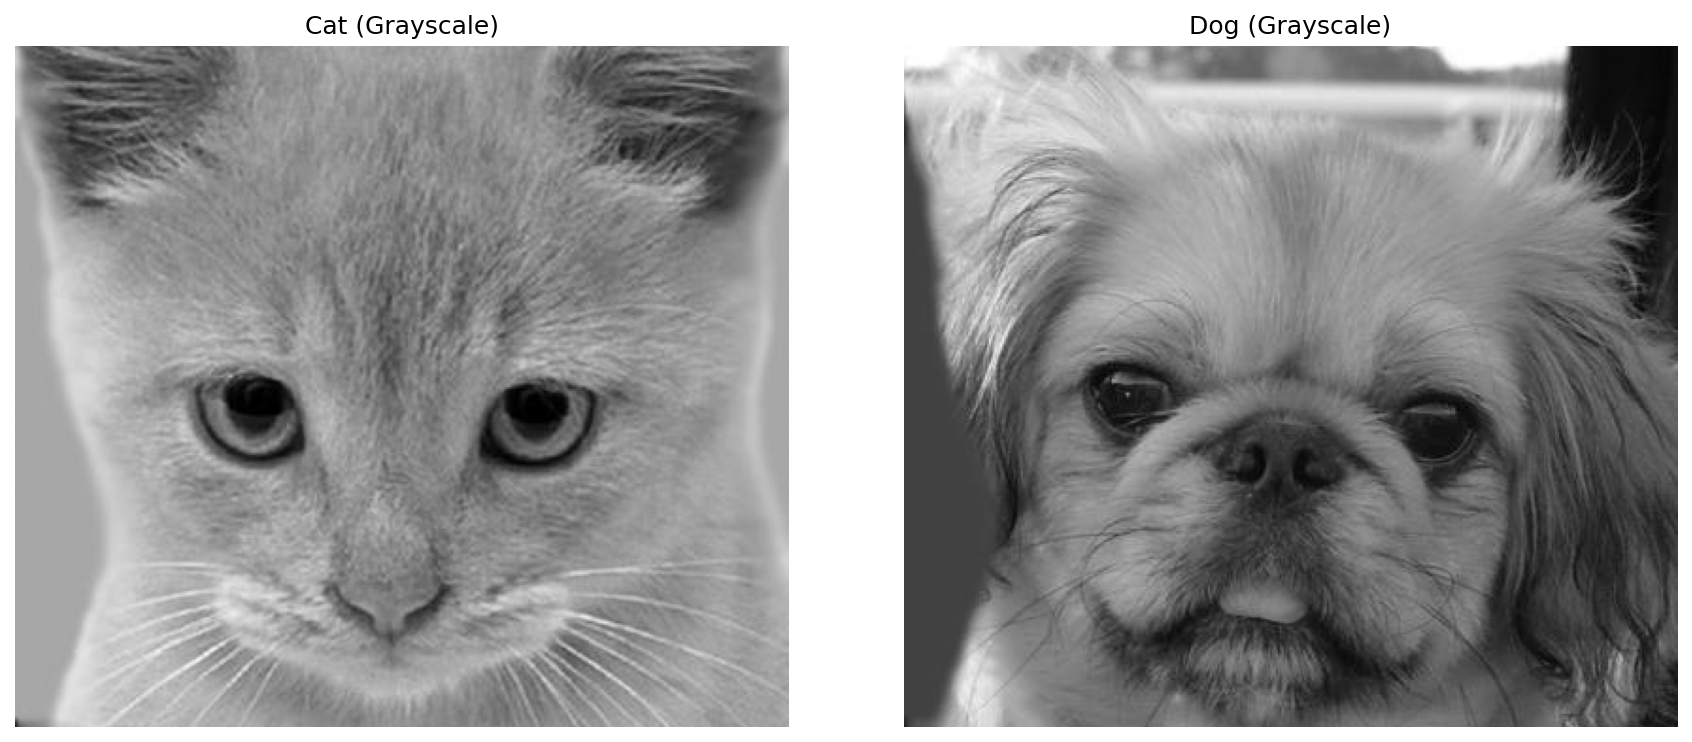
\includegraphics[width=0.8\textwidth]{report_images/01_original_images.png}
    \caption{Original grayscale images: (a) Cat and (b) Dog}
    \label{fig:original_images}
\end{figure}

\begin{figure}[H]
    \centering
    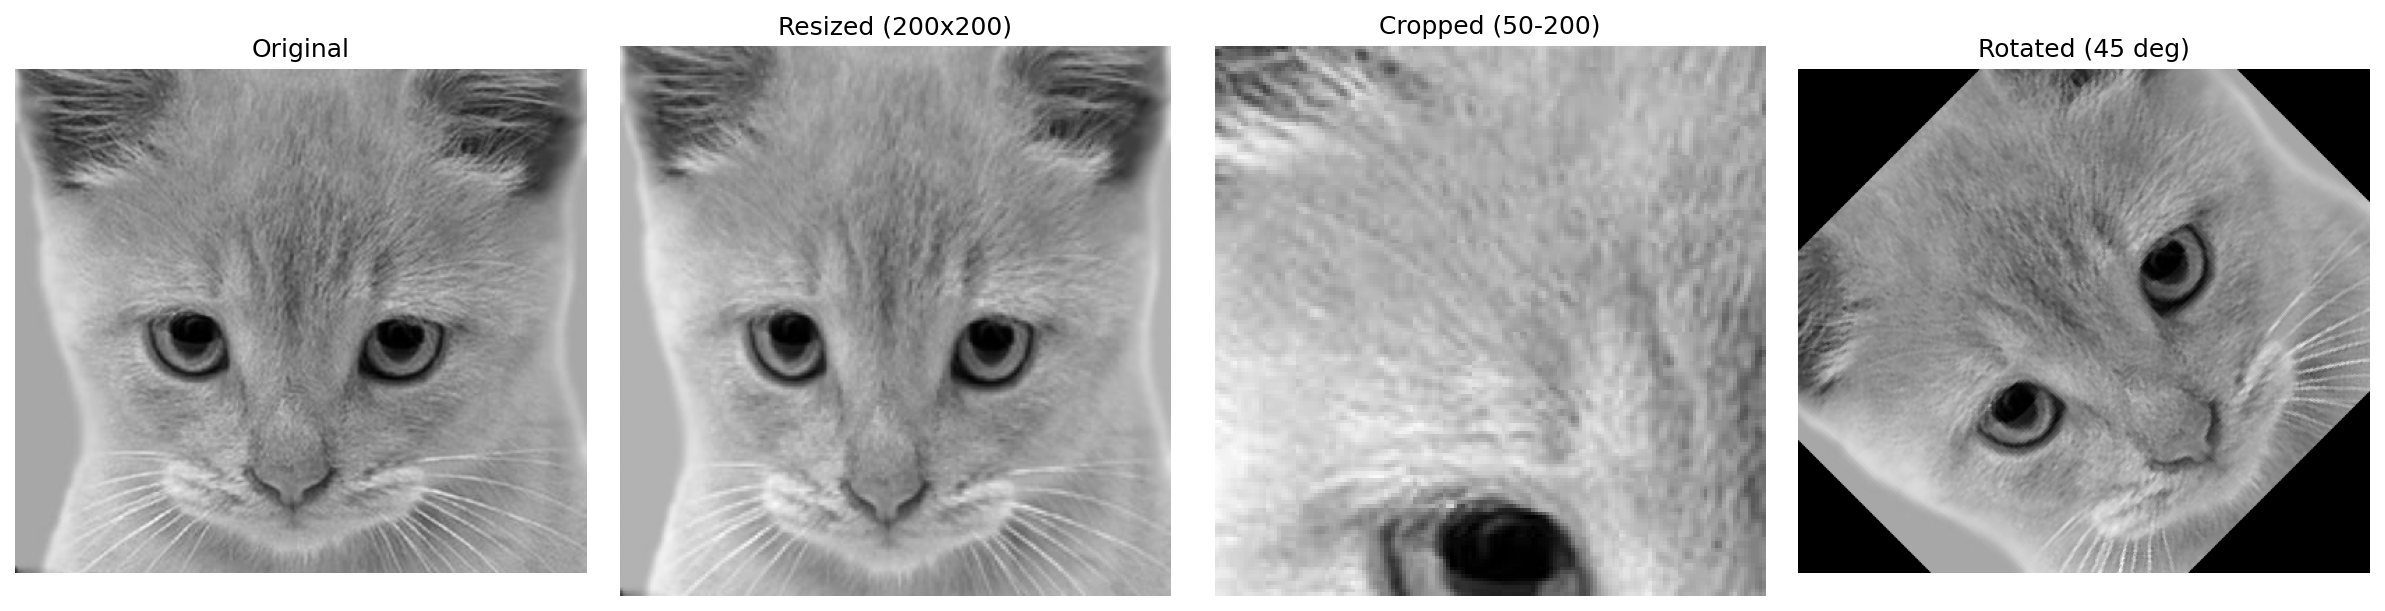
\includegraphics[width=0.8\textwidth]{report_images/02_image_operations.png}
    \caption{Basic image operations: (a) Original, (b) Resized 200$\times$200, (c) Cropped, (d) Rotated 45°}
    \label{fig:image_operations}
\end{figure}

\begin{figure}[H]
    \centering
    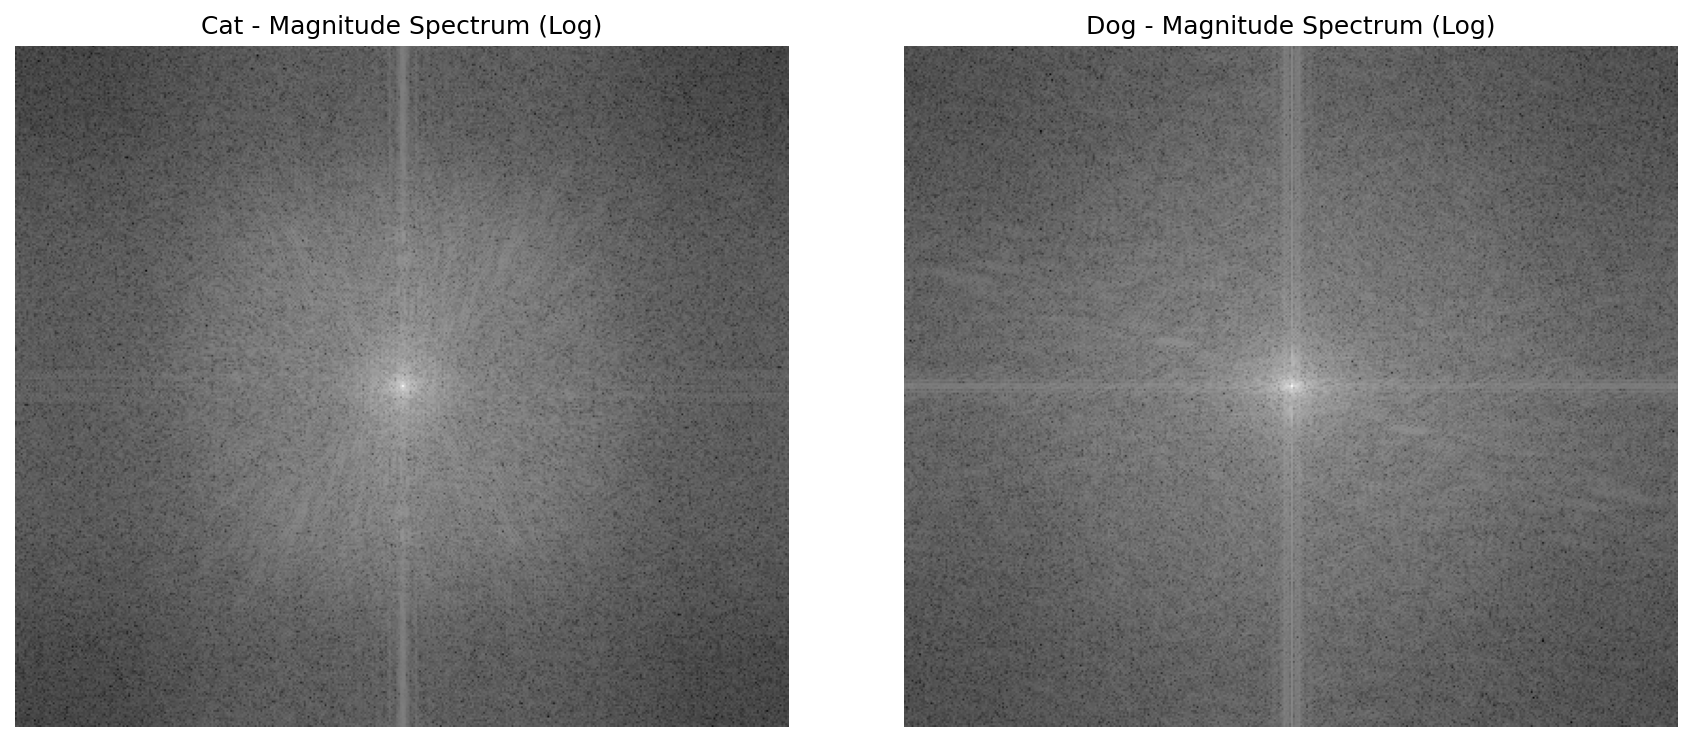
\includegraphics[width=0.8\textwidth]{report_images/03_magnitude_spectra.png}
    \caption{2D DFT Magnitude Spectra: (a) Cat image frequency content, (b) Dog image frequency content}
    \label{fig:magnitude_spectra}
\end{figure}

\begin{figure}[H]
    \centering
    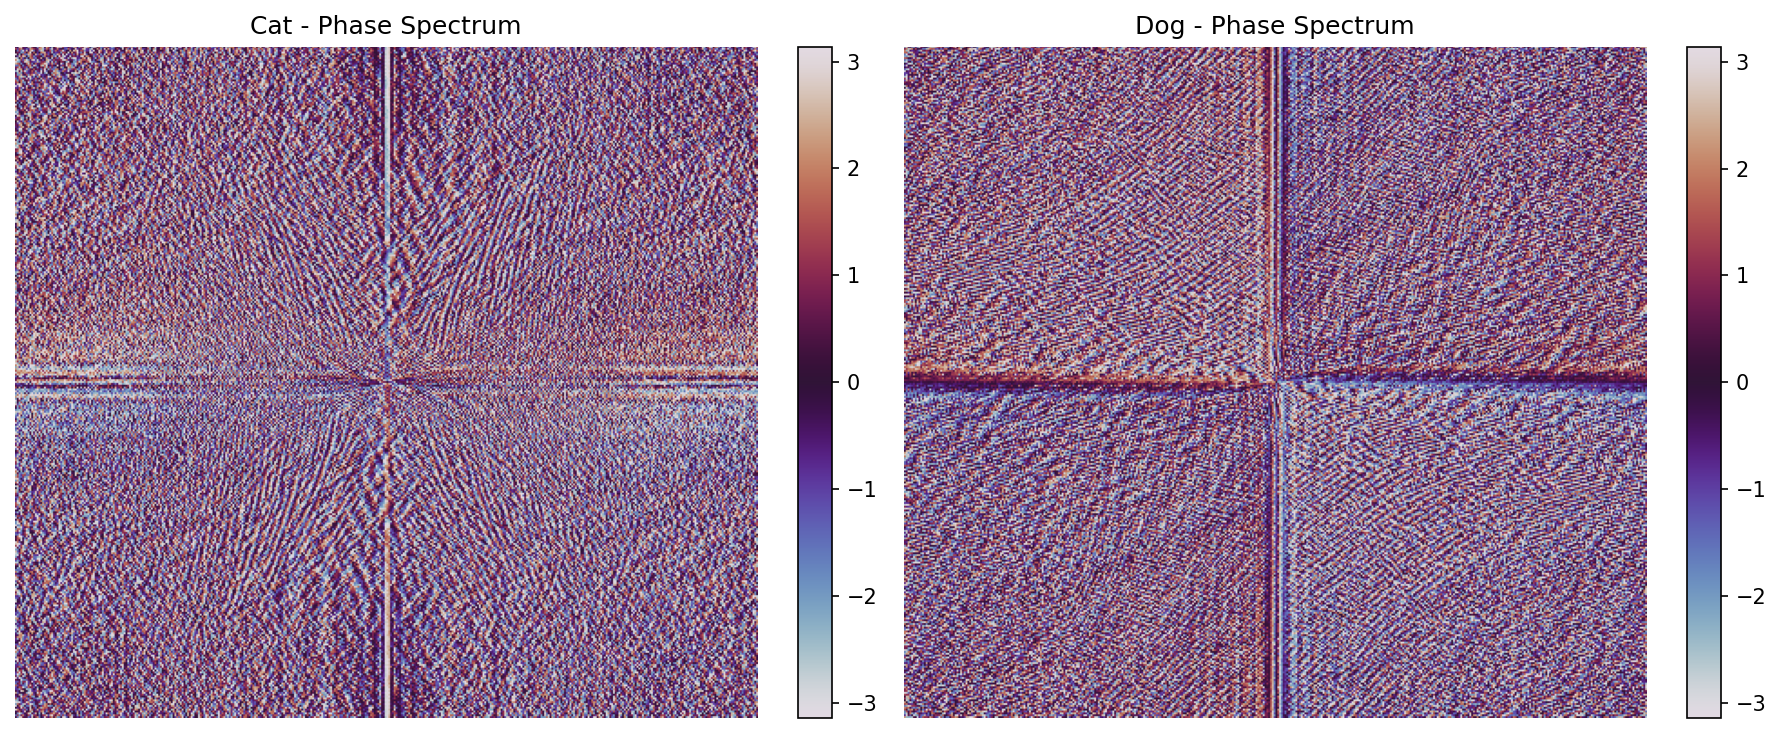
\includegraphics[width=0.8\textwidth]{report_images/04_phase_spectra.png}
    \caption{Phase spectra showing phase angle distribution: (a) Cat, (b) Dog}
    \label{fig:phase_spectra}
\end{figure}

\bigskip
\subsection{Rotation Property of the Fourier Transform}
An important property of the Fourier transform is that rotation in the spatial domain results in an equivalent rotation in the frequency domain:

\bigskip
\begin{equation}
    \text{If } f_r(x,y) = f(x\cos\theta + y\sin\theta, -x\sin\theta + y\cos\theta)
    \quad\Rightarrow\quad
    F_r(u,v) = F(u\cos\theta + v\sin\theta, -u\sin\theta + v\cos\theta)
    \label{eq:rotation_property}
\end{equation}

\bigskip
This can be verified by comparing the magnitude spectrum of the original image with that of a 90° rotated version. The energy distribution remains identical, with only the orientation changing.

\begin{figure}[H]
    \centering
    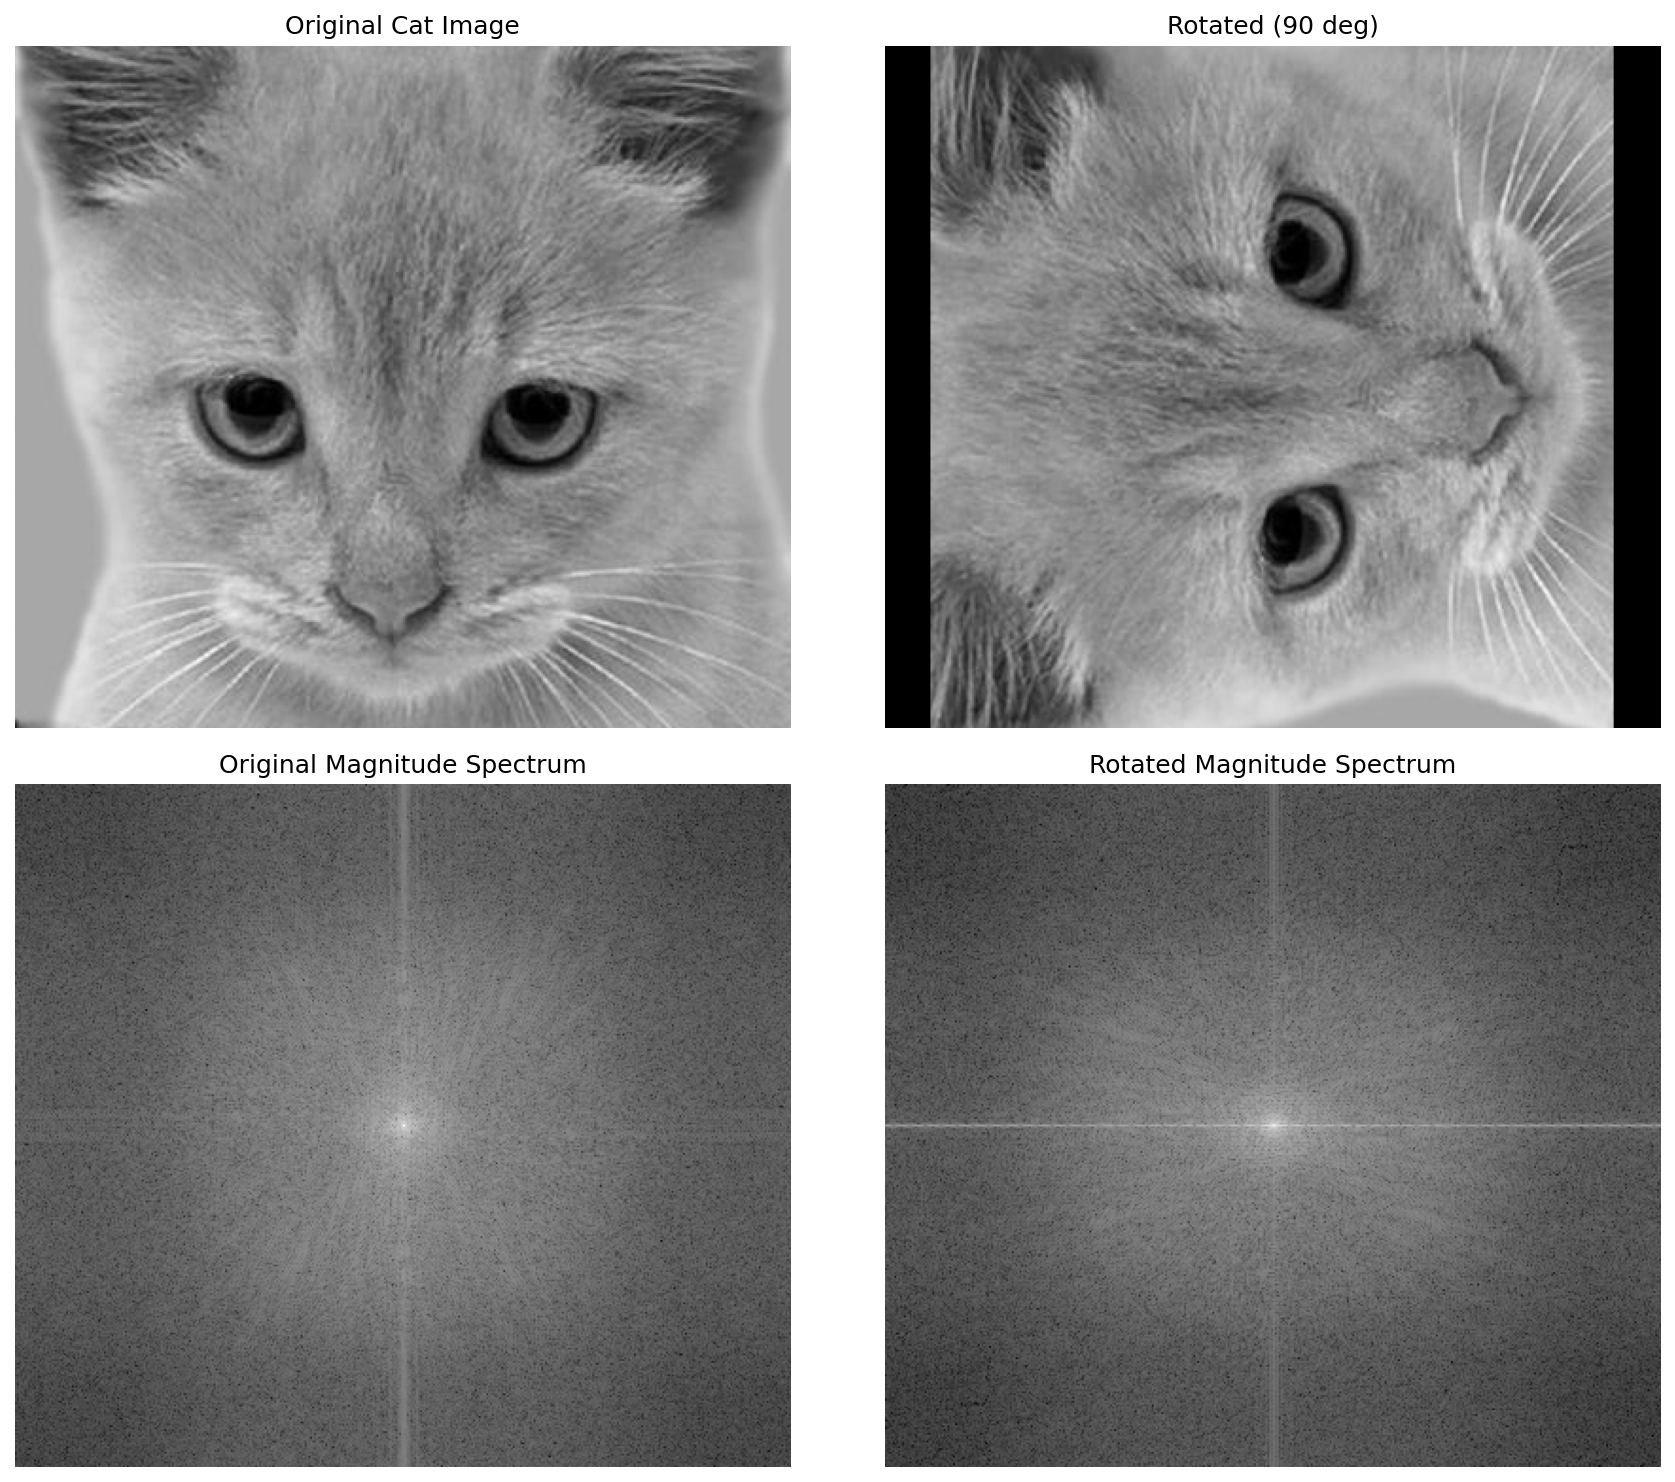
\includegraphics[width=0.9\textwidth]{report_images/07_rotation_comparison.png}
    \caption{Rotation property demonstration: (a) Original Cat image, (b) 90° Anti-clockwise rotated, (c) Original magnitude spectrum, (d) Rotated magnitude spectrum showing equivalent rotation}
    \label{fig:rotation_comparison}
\end{figure}

\bigskip
\textbf{Observations:}
\begin{enumerate}
    \item The magnitude spectrum of the rotated image is rotated by the same angle as the spatial transformation
    \item The total energy (sum of squared magnitudes) is preserved --- demonstrating Parseval's theorem in 2D
    \item Only the orientation changes, not the magnitude distribution: $|F(u,v)| = |F_r(u,v)|$
\end{enumerate}

\bigskip
\subsection{Frequency Domain Filtering}
Frequency domain filtering operates by modifying the Fourier transform coefficients before applying the inverse transform. For an ideal filter, the transfer function is defined as:

\bigskip
\textbf{Ideal Low-Pass Filter (LPF):}
\begin{equation}
    H_{LPF}(u,v) =
    \begin{cases}
        1 & \text{if } \sqrt{u^2 + v^2} \leq D_0 \\
        0 & \text{otherwise}
    \end{cases}
    \label{eq:lpf}
\end{equation}

\bigskip
\textbf{Ideal High-Pass Filter (HPF):}
\begin{equation}
    H_{HPF}(u,v) =
    \begin{cases}
        0 & \text{if } \sqrt{u^2 + v^2} \leq D_0 \\
        1 & \text{otherwise}
    \end{cases}
    \label{eq:hpf}
\end{equation}

\bigskip
Where $D_0$ is the cutoff frequency (in pixels from the center). The filtered image is obtained by:

\bigskip
\begin{equation}
    g(x,y) = \mathcal{F}^{-1}\{F(u,v) \cdot H(u,v)\}
    \label{eq:filtering}
\end{equation}

\bigskip
We demonstrate filtering at multiple cutoff values:
\begin{itemize}
    \item \textbf{Conservative (25\%)}: $D_0 = \frac{\min(M,N)}{4}$ --- Subtle blur
    \item \textbf{Default (12.5\%)}: $D_0 = \frac{\min(M,N)}{8}$ --- Moderate effect
    \item \textbf{Aggressive (6.25\%)}: $D_0 = \frac{\min(M,N)}{16}$ --- Strong blur
\end{itemize}

\begin{figure}[H]
    \centering
    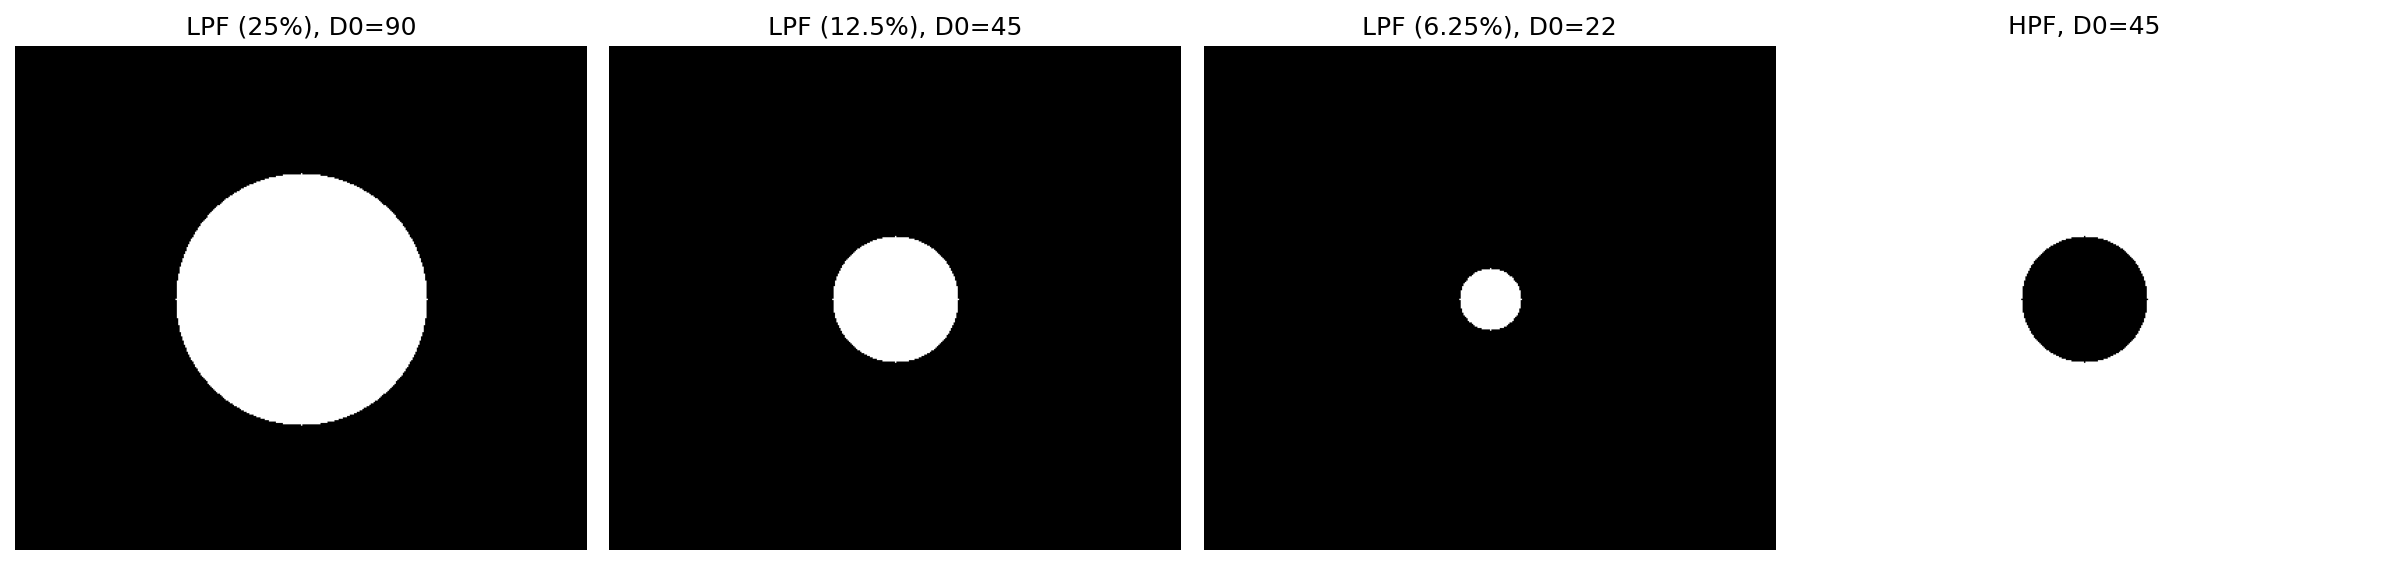
\includegraphics[width=0.9\textwidth]{report_images/05_filter_masks.png}
    \caption{Filter transfer functions at multiple cutoffs: LPF at 25\%, 12.5\%, 6.25\% and HPF at 12.5\%}
    \label{fig:filter_masks}
\end{figure}

\begin{figure}[H]
    \centering
    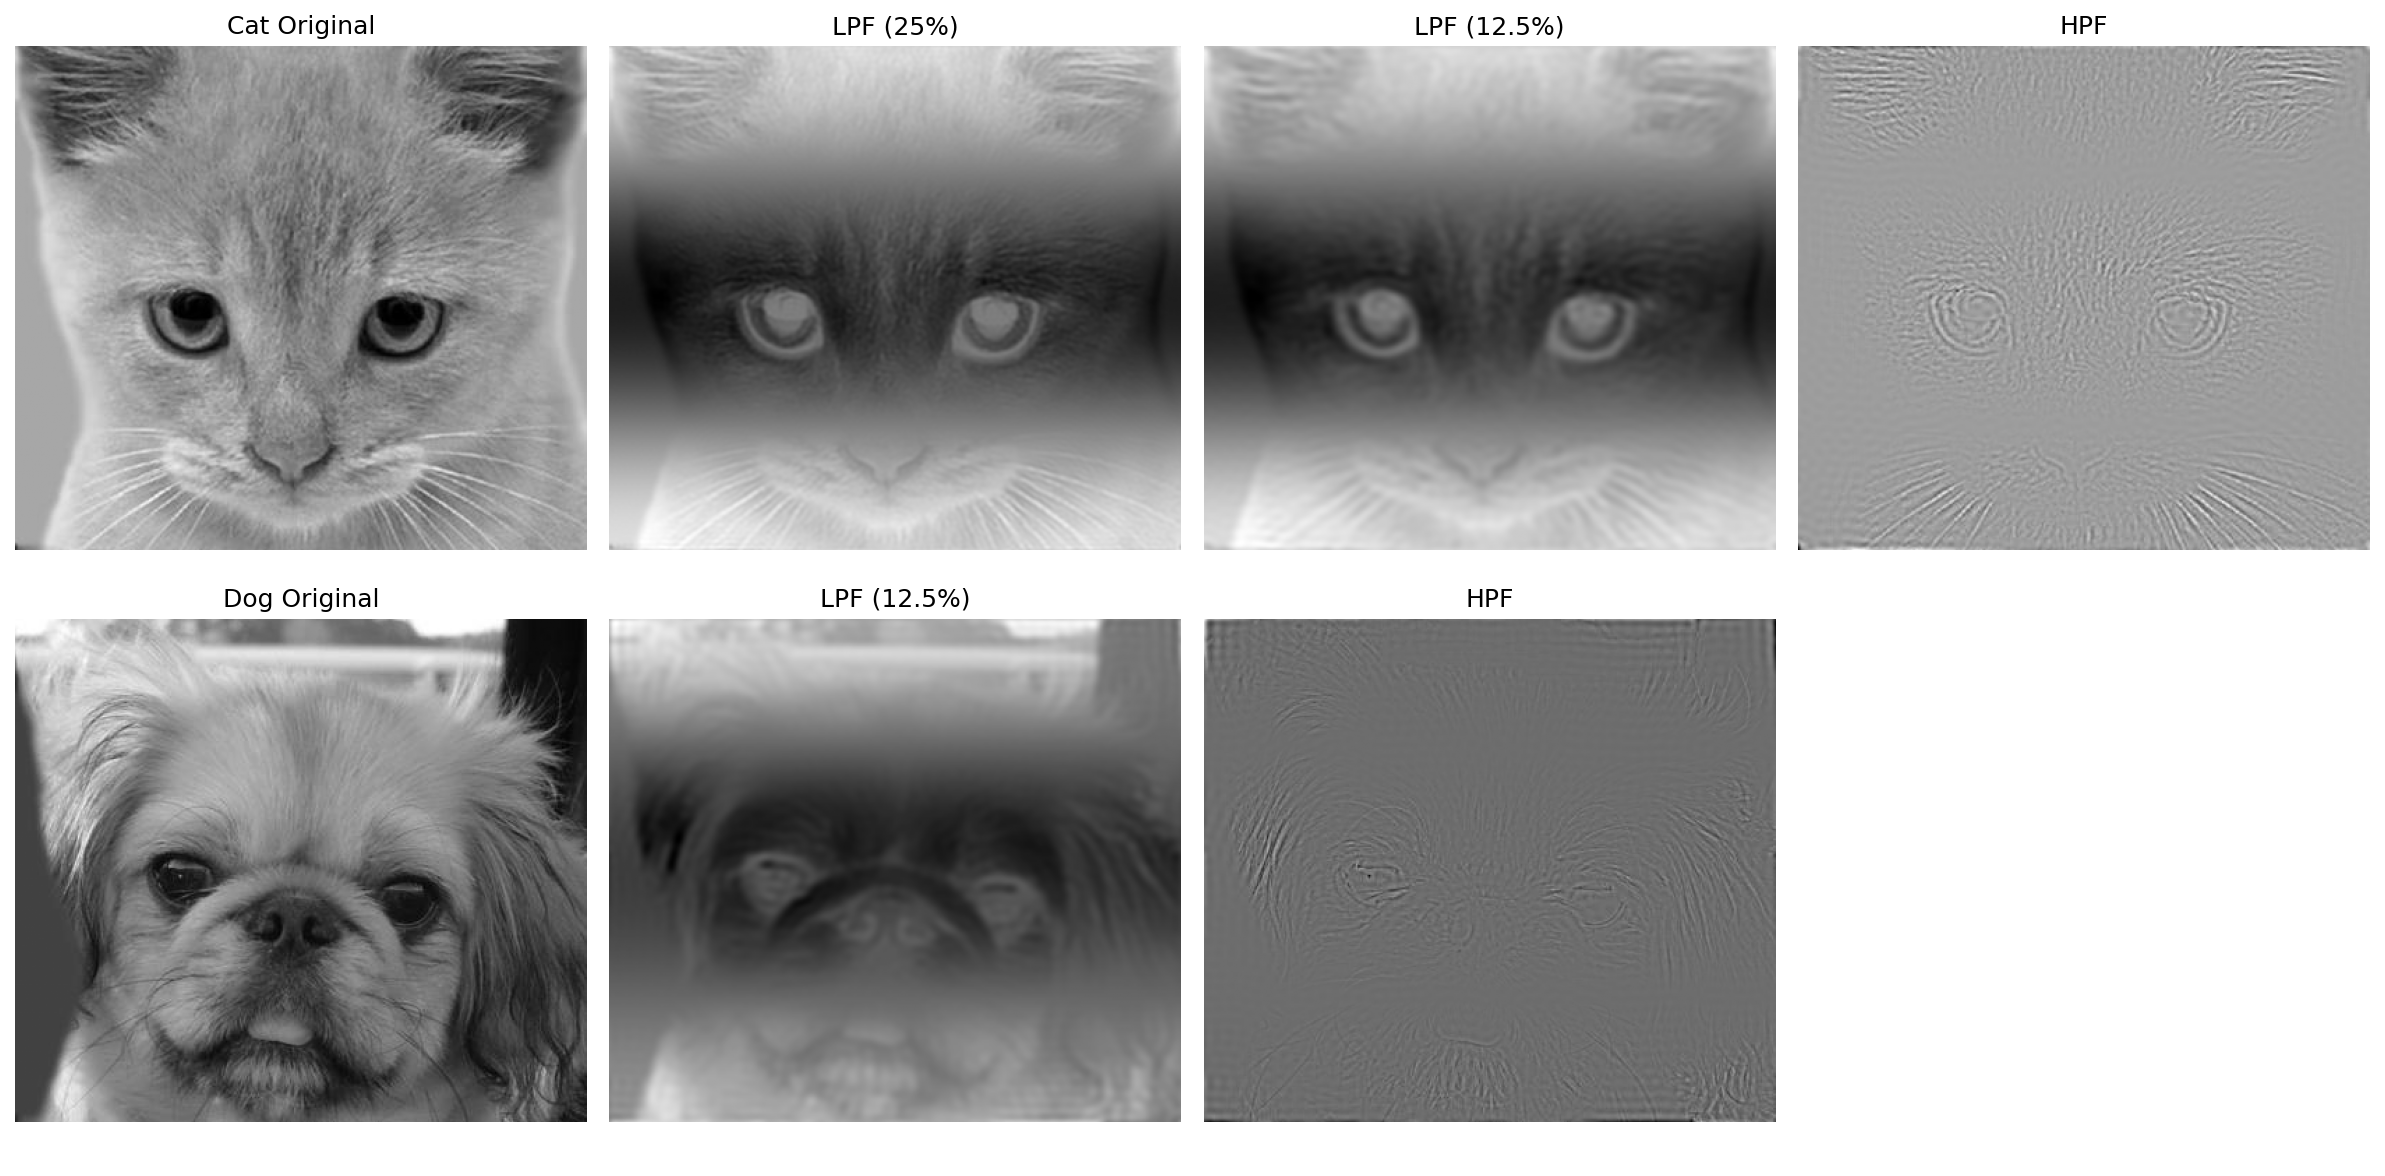
\includegraphics[width=0.9\textwidth]{report_images/06_filtering_results.png}
    \caption{Frequency filtering results: Comparing LPF effects at different cutoffs and HPF edge enhancement}
    \label{fig:filtering_results}
\end{figure}

\bigskip
\textbf{Key Observations:}
\begin{itemize}
    \item \textbf{LPF Effect}: Removes high-frequency components (details), resulting in a blurred/smoothed image
    \item \textbf{HPF Effect}: Removes low-frequency components (smooth regions), resulting in edge enhancement
    \item Lower cutoff values produce stronger filtering effects
\end{itemize}

\bigskip
\subsection{Frequency Mixer: Creative Image Fusion}
The Frequency Mixer demonstrates an advanced application of frequency domain processing by combining frequency components from two different images. This creates hybrid images where:

\bigskip
\begin{itemize}
    \item One image provides \textbf{LOW frequencies} (overall structure/shape)
    \item The other image provides \textbf{HIGH frequencies} (fine details/texture)
\end{itemize}

\bigskip
The mathematical formulation is:

\bigskip
\begin{equation}
    F_{mixed}(u,v) = F_A(u,v) \cdot H_{LPF}(u,v) + F_B(u,v) \cdot H_{HPF}(u,v)
    \label{eq:mixer}
\end{equation}

\bigskip
Equivalently, in spatial domain:

\bigskip
\begin{equation}
    f_{mixed}(x,y) = \mathcal{F}^{-1}\{F_A \cdot H_{LPF} + F_B \cdot H_{HPF}\}
    \label{eq:mixer_spatial}
\end{equation}

\bigskip
Where:
\begin{itemize}
    \item $F_A$ = FFT of image providing structure (Image A)
    \item $F_B$ = FFT of image providing details (Image B)
    \item $H_{LPF}$ = Low-pass filter mask (passes structure)
    \item $H_{HPF}$ = High-pass filter mask (passes details)
\end{itemize}

\bigskip
The 2D transfer function plots visualize which frequency regions are extracted from each source image:

\bigskip
\begin{figure}[H]
    \centering
    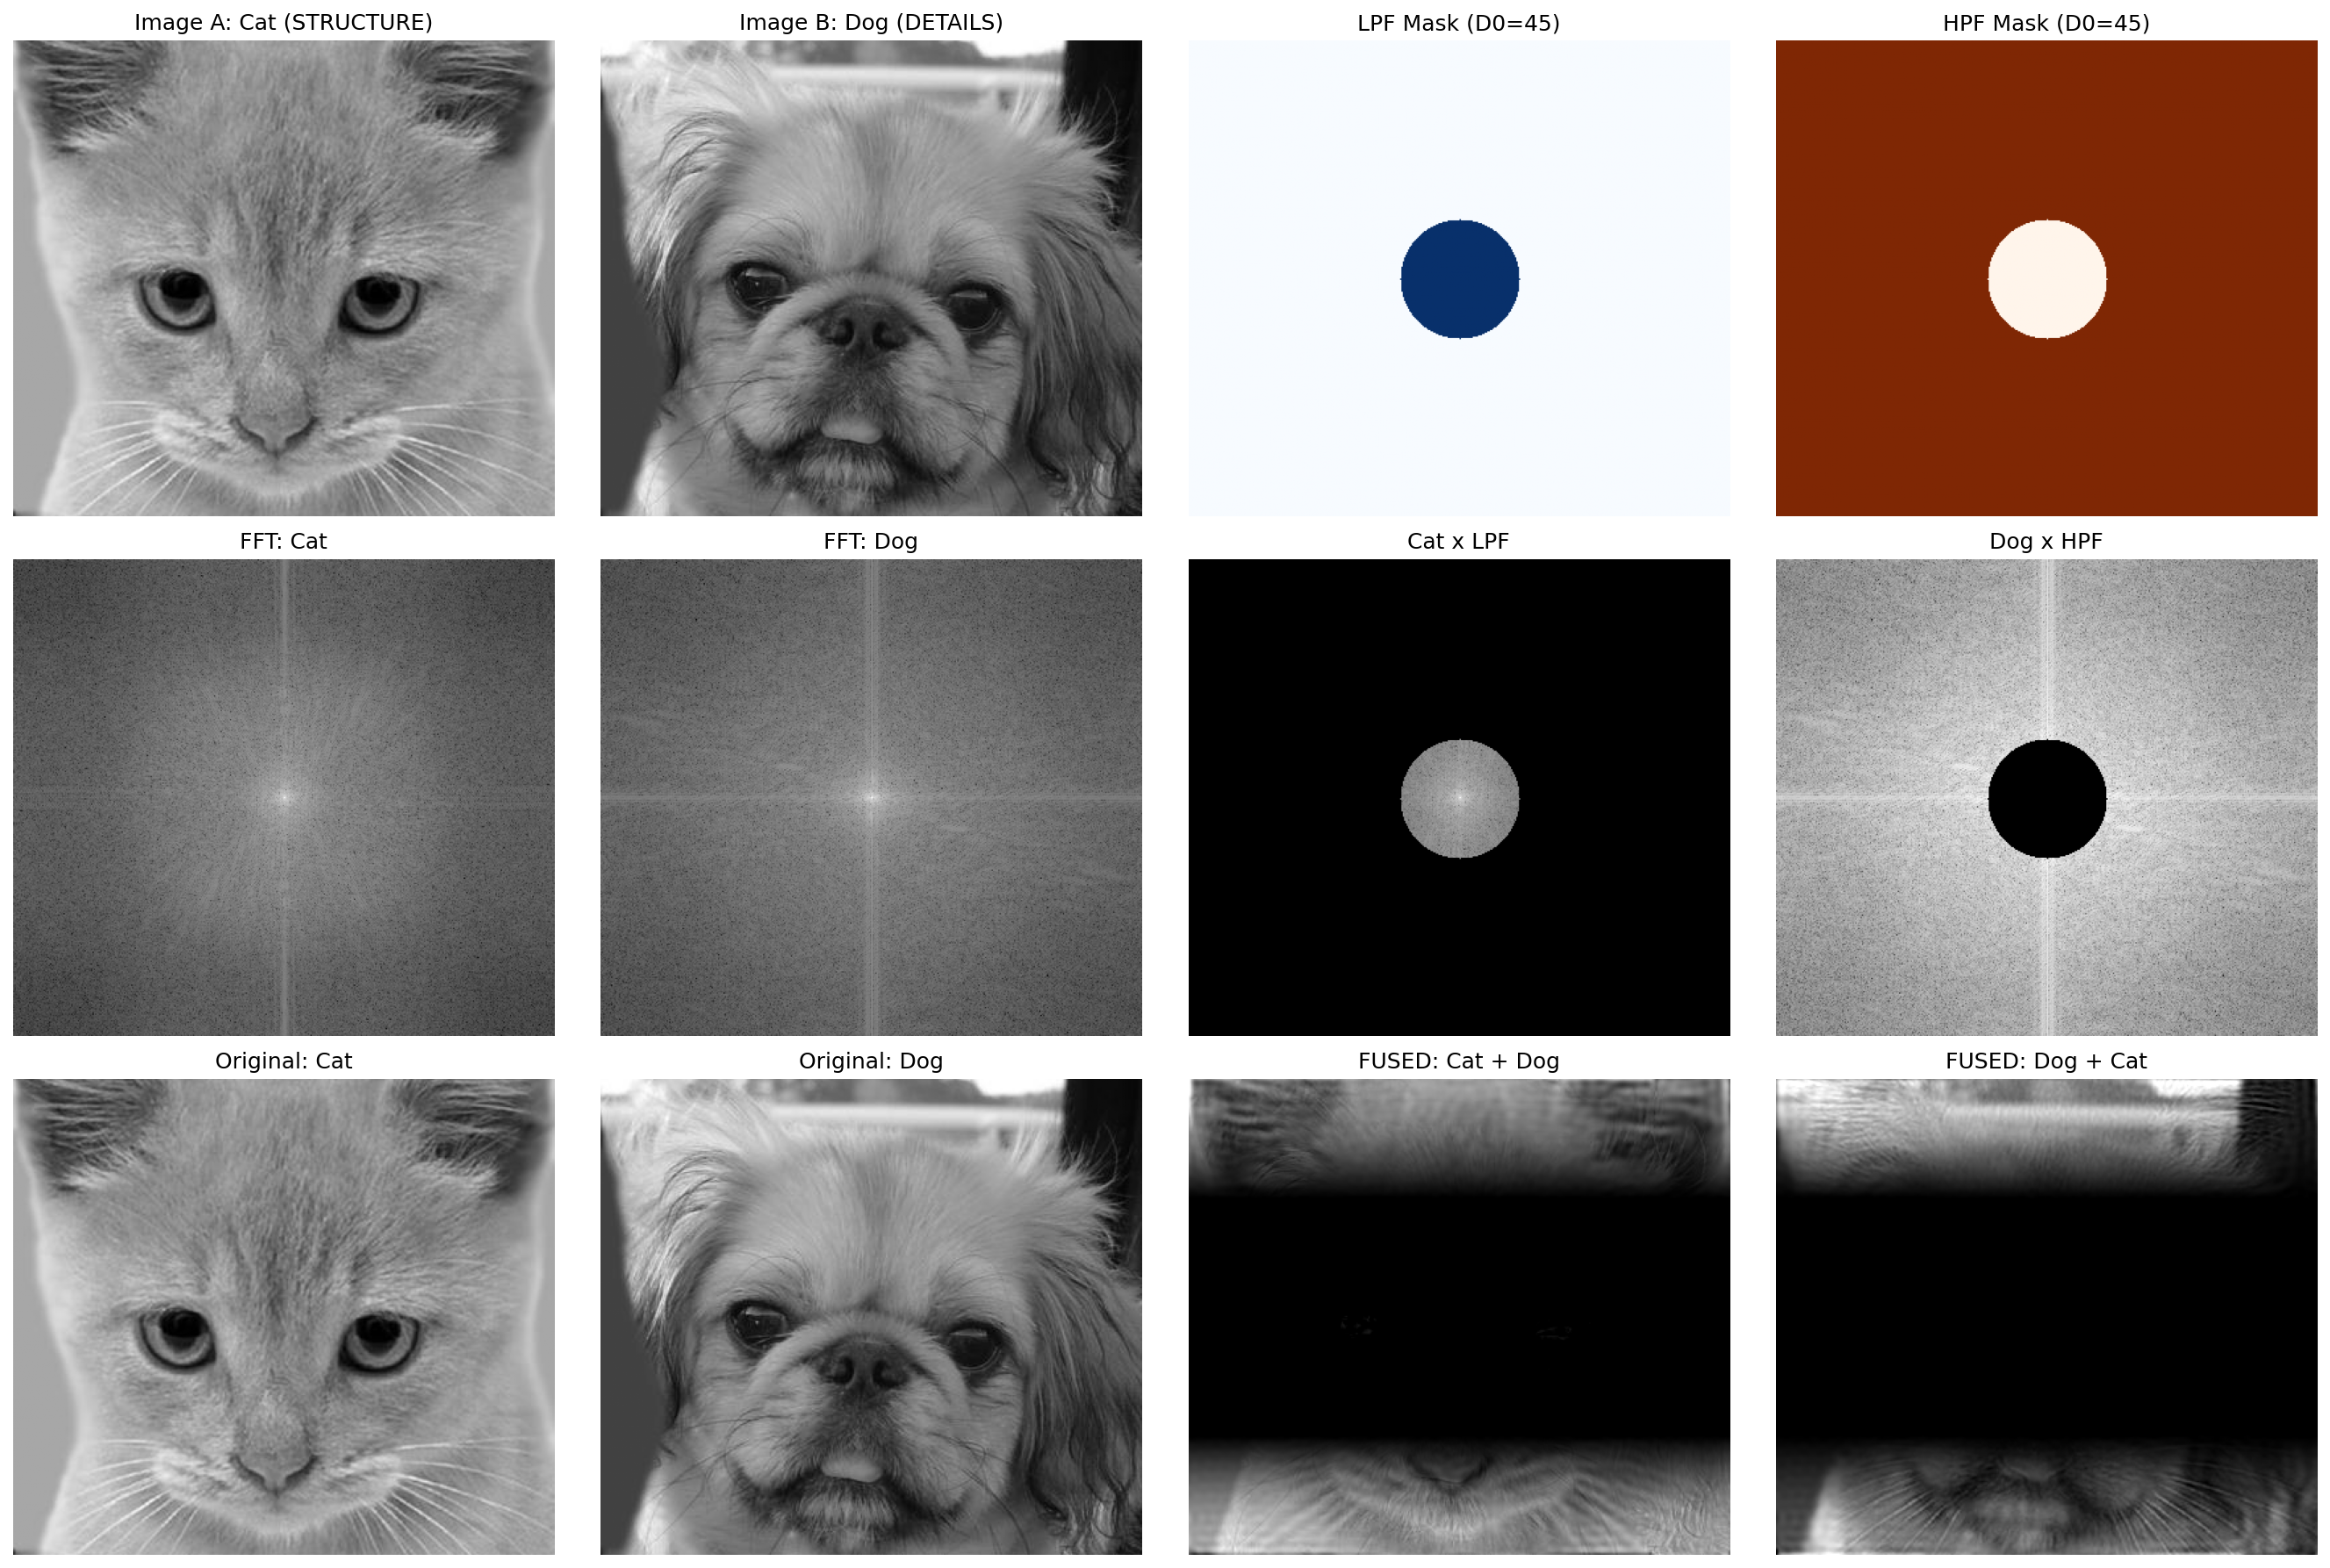
\includegraphics[width=1.0\textwidth]{report_images/08_frequency_mixer.png}
    \caption{Frequency Mixer system: Source images (Cat, Dog), Filter masks (LPF for structure, HPF for details), FFT analysis, and final fused results}
    \label{fig:frequency_mixer_system}
\end{figure}

\bigskip
\begin{figure}[H]
    \centering
    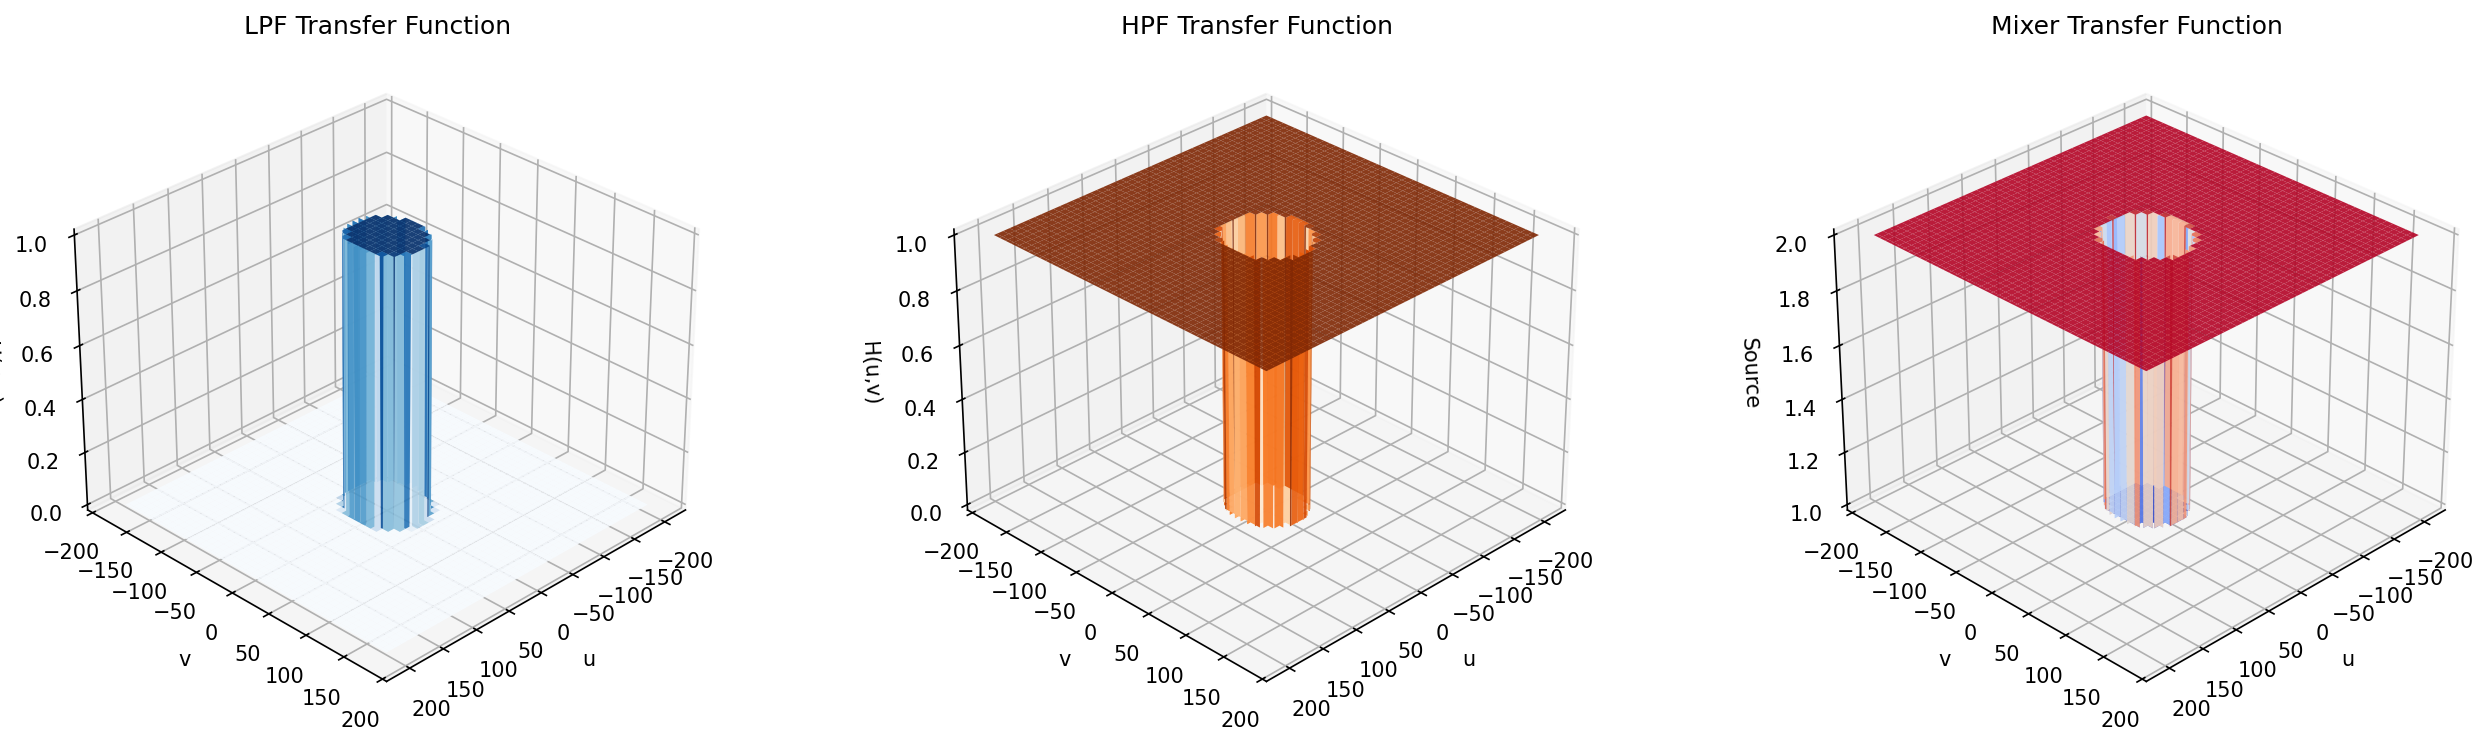
\includegraphics[width=0.9\textwidth]{report_images/09_3d_transfer_functions.png}
    \caption{2D Transfer Functions as 3D surfaces: (a) LPF showing structure filter, (b) HPF showing details filter, (c) Combined mixer showing source regions}
    \label{fig:transfer_functions_3d}
\end{figure}

\bigskip
\textbf{Frequency Mixer Transfer Function Summary:}

\begin{table}[H]
    \centering
    \begin{tabular}{|c|c|c|c|}
        \hline
        \textbf{Region} & \textbf{Radius} & \textbf{Passes} & \textbf{Contains} \\
        \hline
        Low Frequency & $r \leq D_0$ & LPF & Structure \\
        \hline
        High Frequency & $r > D_0$ & HPF & Details \\
        \hline
    \end{tabular}
    \caption{Frequency Mixer Transfer Function Parameters}
    \label{tab:mixer_params}
\end{table}

\bigskip
\textbf{Results:}
\begin{itemize}
    \item \textbf{Mix 1}: Cat structure + Dog details = Cat's overall shape with dog's texture
    \item \textbf{Mix 2}: Dog structure + Cat details = Dog's overall shape with cat's texture
\end{itemize}

\bigskip
\textbf{Applications of Frequency Mixing:}
\begin{itemize}
    \item Image blending and artistic effects
    \item Medical imaging (CT + MRI fusion)
    \item Multi-focus photography combination
    \item Texture transfer between images
\end{itemize}

\bigskip
\section{Part B: Audio Signal Processing}

\subsection{Audio Loading and Metadata}
The audio file \texttt{song\_with\_2piccolo.wav} is loaded using the Librosa library:

\bigskip
\begin{verbatim}
y, sr = librosa.load(audio_path, sr=None)
duration = len(y) / sr
\end{verbatim}

\bigskip
Where:
\begin{itemize}
    \item $y$ = Audio signal array
    \item $sr$ = Sampling rate (Hz)
    \item $duration$ = Total audio duration in seconds
\end{itemize}

\bigskip
\subsection{Audio Restoration Using Frequency Filtering}
Applying the same frequency domain filtering principles to audio signals enables noise reduction and audio enhancement. We apply FFT-based filtering:

\bigskip
\begin{equation}
    Y(\omega) = \mathcal{F}\{y(t)\}
    \label{eq:audio_fft}
\end{equation}

\bigskip
\begin{equation}
    Y_{filtered}(\omega) = Y(\omega) \cdot H(\omega)
    \label{eq:audio_filtered}
\end{equation}

\bigskip
\begin{equation}
    y_{filtered}(t) = \mathcal{F}^{-1}\{Y_{filtered}(\omega)\}
    \label{eq:audio_ifft}
\end{equation}

\bigskip
Where $H(\omega)$ is the frequency response of the chosen filter.

\bigskip
The following audio files are generated:
\begin{itemize}
    \item \texttt{audio\_original.wav} --- Original audio signal
    \item \texttt{audio\_LPF\_restored.wav} --- Low-pass filtered (removes high-frequency noise)
    \item \texttt{audio\_HPF\_restored.wav} --- High-pass filtered (removes low-frequency rumble)
\end{itemize}

\begin{figure}[H]
    \centering
    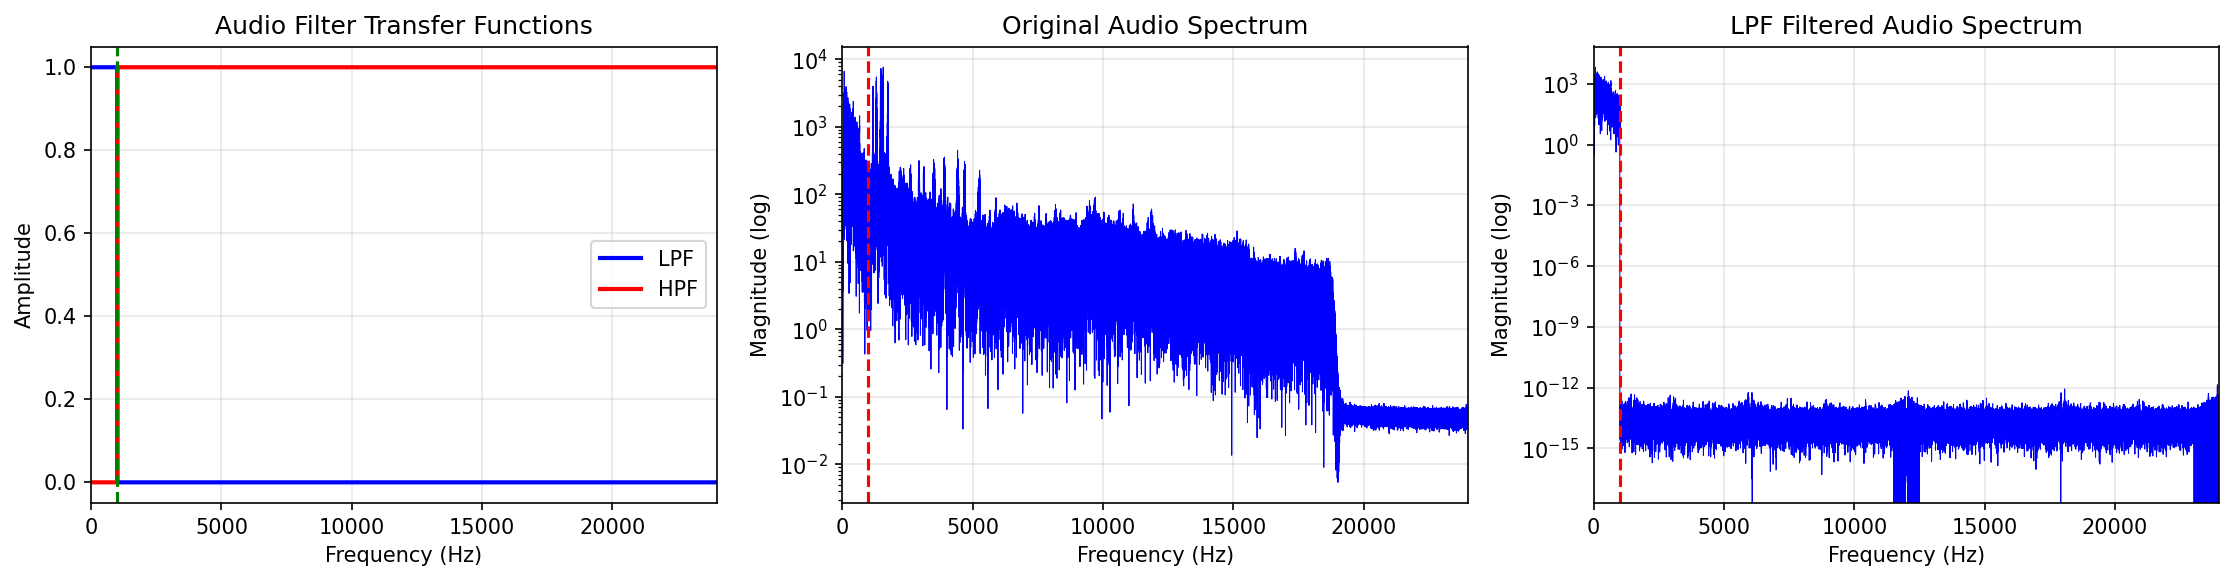
\includegraphics[width=0.9\textwidth]{report_images/10_audio_filtering.png}
    \caption{Audio frequency domain filtering: (a) Filter transfer functions, (b) Original audio spectrum, (c) LPF filtered spectrum}
    \label{fig:audio_filtering}
\end{figure}

\bigskip
\subsection{Audio Waveform Visualization}
The audio waveform represents amplitude variation over time:

\bigskip
\begin{figure}[H]
    \centering
    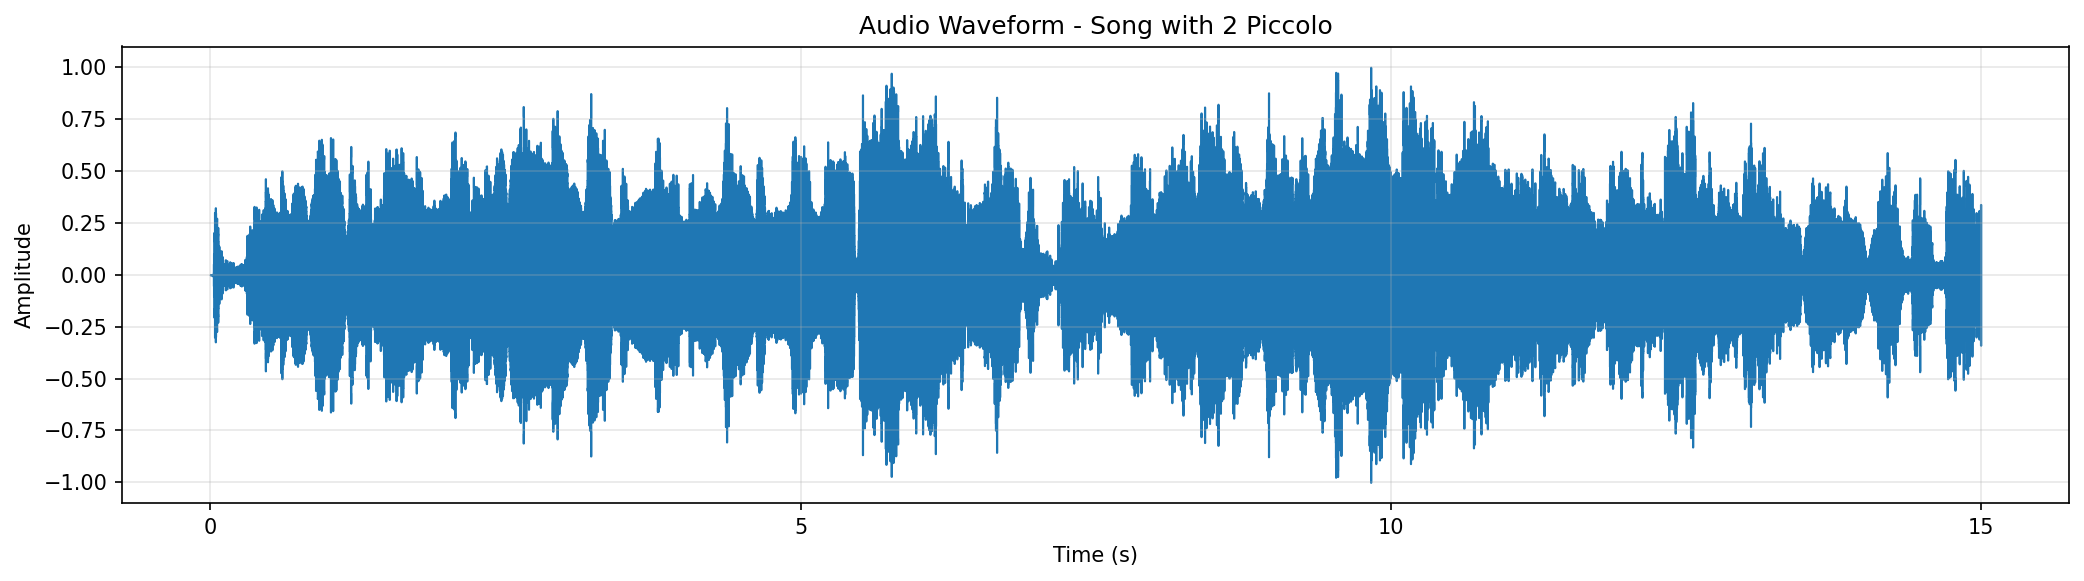
\includegraphics[width=1.0\textwidth]{report_images/11_audio_waveform.png}
    \caption{Audio waveform showing amplitude variation over time for the piccolo recording}
    \label{fig:audio_waveform}
\end{figure}

\bigskip
\subsection{Short-Time Fourier Transform (STFT) and Spectrogram}
The STFT provides time-frequency analysis by applying the DFT to overlapping windowed segments of the signal:

\bigskip
\begin{equation}
    D(k,l) = \sum_{n=0}^{N-1} x(n) \cdot w(n-lR) \cdot e^{-j2\pi kn/N}
    \label{eq:stft}
\end{equation}

\bigskip
Where:
\begin{itemize}
    \item $w(n)$ = Analysis window function
    \item $R$ = Hop size (advance between frames)
    \item $N$ = FFT window size
    \item $(k,l)$ = Frequency bin and time frame indices
\end{itemize}

\bigskip
The spectrogram visualizes the STFT magnitude on a time-frequency plane:

\bigskip
\begin{equation}
    S_{dB}(k,l) = 20 \cdot \log_{10}\left(\frac{|D(k,l)|}{|D_{max}|}\right)
    \label{eq:spectrogram_db}
\end{equation}

\bigskip
\begin{figure}[H]
    \centering
    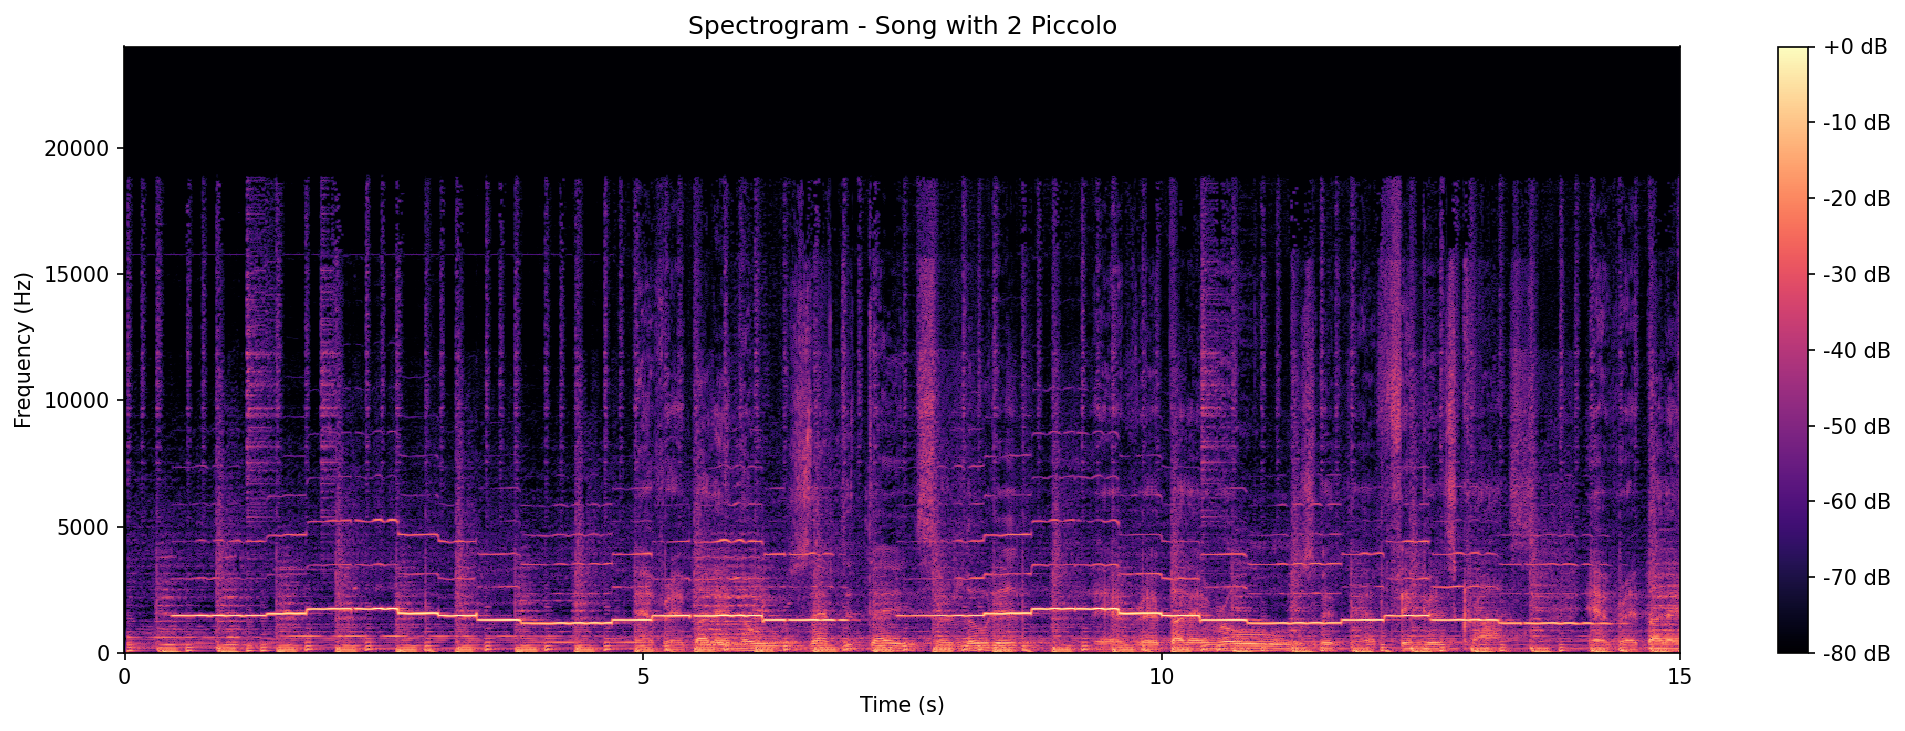
\includegraphics[width=1.0\textwidth]{report_images/12_spectrogram.png}
    \caption{Spectrogram showing frequency content over time. Brighter colors indicate higher energy at that frequency.}
    \label{fig:spectrogram}
\end{figure}

\bigskip
\subsection{Spectral Analysis: Dominant Frequency Identification}
The power spectral density is computed by averaging the STFT magnitude across all time frames:

\bigskip
\begin{equation}
    P(f) = \frac{1}{T}\sum_{l=0}^{T-1}|D(f,l)|^2
    \label{eq:psd}
\end{equation}

\bigskip
Peak detection identifies the dominant harmonic frequencies in the piccolo recording:

\bigskip
\begin{figure}[H]
    \centering
    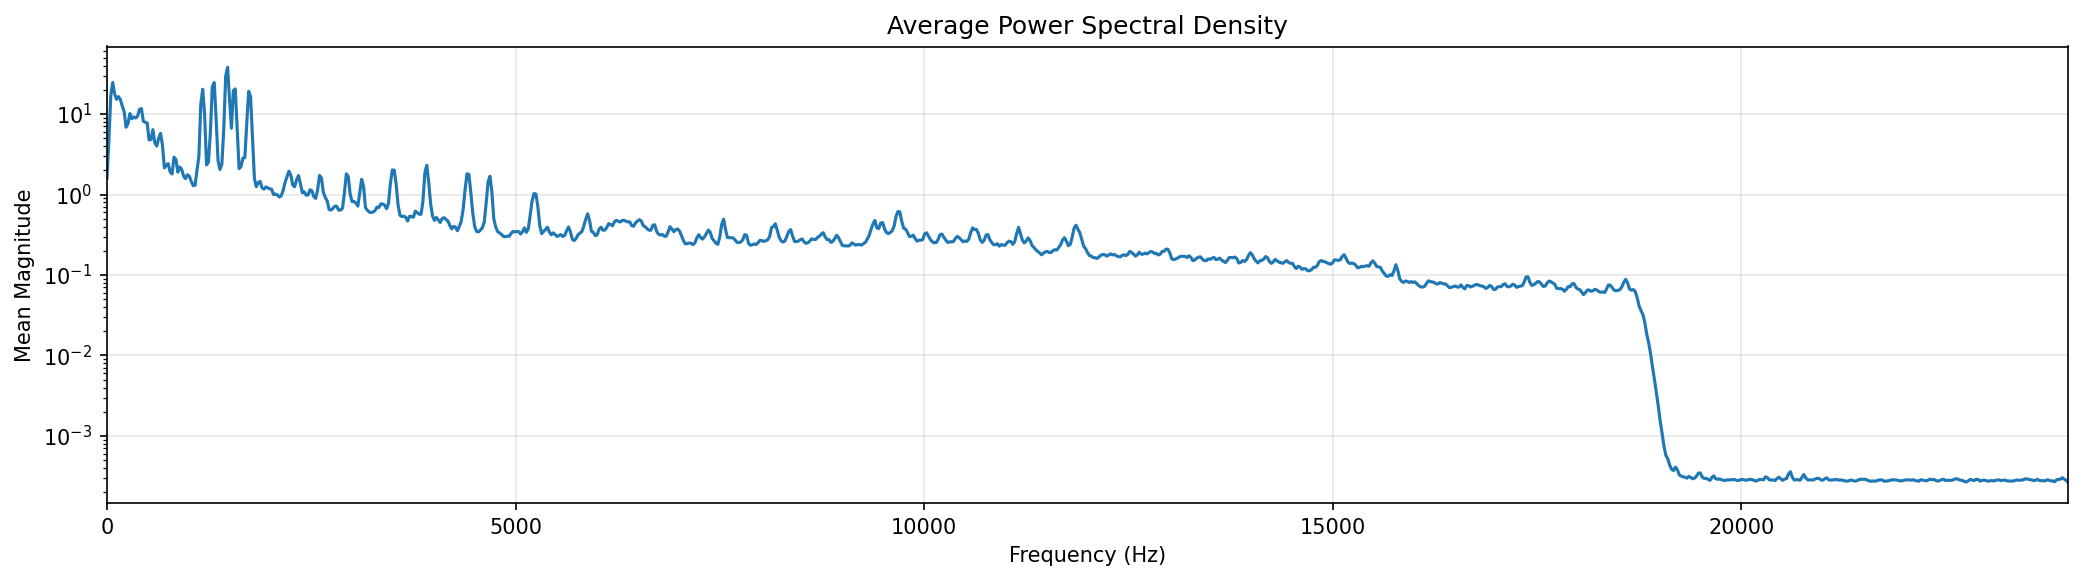
\includegraphics[width=1.0\textwidth]{report_images/13_power_spectrum.png}
    \caption{Average power spectral density showing dominant frequency components}
    \label{fig:psd}
\end{figure}

\bigskip
The top 10 dominant frequencies are extracted, with most falling in the piccolo range of 500 Hz to 4000 Hz.

\bigskip
\section{Results and Discussion}

\subsection{Image Processing Results}
The frequency filtering experiments demonstrate clear visible effects:

\bigskip
\begin{table}[H]
    \centering
    \begin{tabular}{|c|c|p{5cm}|}
        \hline
        \textbf{Filter} & \textbf{Cutoff} & \textbf{Observed Effect} \\
        \hline
        LPF Conservative & 25\% & Subtle blur, details still visible \\
        \hline
        LPF Default & 12.5\% & Moderate blur, fur texture softened \\
        \hline
        LPF Aggressive & 6.25\% & Strong blur, major features only \\
        \hline
        HPF Default & 12.5\% & Edge enhancement, smooth areas dark \\
        \hline
    \end{tabular}
    \caption{Summary of image filtering results}
    \label{tab:image_results}
\end{table}

\bigskip
The Frequency Mixer successfully creates hybrid images:
\begin{itemize}
    \item Cat structure + Dog details: Cat's outline combined with dog's fine texture
    \item Dog structure + Cat details: Dog's outline combined with cat's fine texture
\end{itemize}

\bigskip
\subsection{Audio Processing Results}

\bigskip
\begin{table}[H]
    \centering
    \begin{tabular}{|c|c|p{5cm}|}
        \hline
        \textbf{Metric} & \textbf{Value} & \textbf{Description} \\
        \hline
        Sampling Rate & 48000 Hz & Standard CD quality \\
        \hline
        Duration & Variable & Based on file length \\
        \hline
        LPF Cutoff & 1000 Hz & Removes high-frequency noise \\
        \hline
        HPF Cutoff & 1000 Hz & Removes low-frequency rumble \\
        \hline
    \end{tabular}
    \caption{Audio processing parameters and results}
    \label{tab:audio_results}
\end{table}

\bigskip
\section{Conclusions}
This project successfully demonstrated fundamental signal processing concepts:

\bigskip
\begin{enumerate}
    \item \textbf{2D DFT Analysis}: Fourier transforms reveal frequency content in images
    \item \textbf{Frequency Filtering}: LPF creates blur, HPF enhances edges
    \item \textbf{Rotation Property}: FFT rotates equivalently with spatial rotation
    \item \textbf{Frequency Mixer}: Creative fusion combines structure from one image with details from another
    \item \textbf{Audio Processing}: STFT enables time-frequency analysis for audio signals
    \item \textbf{Audio Restoration}: FFT-based filtering enables noise reduction
\end{enumerate}

\bigskip
The techniques demonstrated have broad applications in image enhancement, computer vision, audio processing, medical imaging, and multimedia signal processing.

\bigskip
\section{Appendix: Mathematical Formulas Summary}

\bigskip
\begin{table}[H]
    \centering
    \begin{tabular}{|c|p{6cm}|}
        \hline
        \textbf{Concept} & \textbf{Formula} \\
        \hline
        2D DFT Forward & $F(u,v) = \sum_{x}\sum_{y} f(x,y) e^{-j2\pi(ux/M+vy/N)}$ \\
        \hline
        2D DFT Inverse & $f(x,y) = \frac{1}{MN}\sum_{u}\sum_{v} F(u,v) e^{j2\pi(ux/M+vy/N)}$ \\
        \hline
        LPF Transfer Function & $H_{LPF} = 1$ if $\sqrt{u^2+v^2} \leq D_0$, else $0$ \\
        \hline
        HPF Transfer Function & $H_{HPF} = 0$ if $\sqrt{u^2+v^2} \leq D_0$, else $1$ \\
        \hline
        Frequency Mixing & $F_{mixed} = F_A \cdot H_{LPF} + F_B \cdot H_{HPF}$ \\
        \hline
        STFT & $D(k,l) = \sum_n x(n)w(n-lR)e^{-j2\pi kn/N}$ \\
        \hline
        Spectrogram (dB) & $S_{dB} = 20\log_{10}(|D|/|D_{max}|)$ \\
        \hline
    \end{tabular}
    \caption{Mathematical formulas summary}
    \label{tab:formulas}
\end{table}

\bigskip
\section*{References}
\begin{itemize}
    \item Gonzalez, R.C. and Woods, R.E. (2008). \textit{Digital Image Processing}. 3rd Edition. Pearson Prentice Hall.
    \item Oppenheim, A.V. and Schafer, R.W. (2010). \textit{Discrete-Time Signal Processing}. 3rd Edition. Pearson.
    \item Librosa Documentation. \url{https://librosa.org/doc/latest/index.html}
    \item NumPy Documentation. \url{https://numpy.org/doc/}
\end{itemize}

\vfill
\begin{center}
\textbf{--- End of Report ---}
\end{center}

\end{document}